\section{Objectives and Experimental Method}
\subsection{Maintainer Exposure Sets}
Let $M$ be the observed usernames and $P_m$ the packages linked to $m$. For an endpoint universe $U$, we construct
\begin{equation}
 E_m=\bigcup_{p\in P_m}\reach_U(p),\qquad
 A_e=\{m\in M:e\in E_m\},
\end{equation}
where $\reach_U(p)$ contains reverse-reachable endpoints of $p$, including its eligible seed endpoint. Repository endpoints are deduplicated across every package and path. We condense strongly connected components and propagate exact integer bitsets through the resulting directed acyclic graph. A separate propagation of source-identity bitsets checks the endpoint incidence relation.

\subsection{Three Quantities for the Same Selection}
For selected identities $S\subseteq M$, distinct endpoint coverage is
\begin{equation}
 C(S)=\left|\bigcup_{m\in S}E_m\right|.
\end{equation}
For repository endpoints, $C$ counts each repository reached by the selection once, regardless of how many selected accounts reach it.

To model source-account hardening, suppose exactly one observed username is selected uniformly as a hypothetical compromise origin. Assume a perfect control prevents that origin when selected, while all other scenarios and graph paths remain unchanged. The proportional reduction in expected endpoint count is then
\begin{equation}
 H(S)=\frac{\sum_{m\in S}|E_m|}{\sum_{m\in M}|E_m|}.
 \label{eq:exposure}
\end{equation}
The uniform prior cancels in the ratio; no compromise probabilities are fitted. Because the numerator adds account-specific reach, sorting by exact $|E_m|$ maximizes $H$ at equal costs. A repository reached by two selected accounts contributes to both scenarios. Selecting one account leaves the other account's paths intact.

Finally, we count endpoints for which every observed source has been selected:
\begin{equation}
 P(S)=\sum_{e\in U}\ind[A_e\ne\varnothing\ \land\ A_e\subseteq S].
 \label{eq:exclusion}
\end{equation}
We call this \emph{all-source exclusion}. Requiring a nonempty $A_e$ prevents credit for missing source evidence. The difference $C(S)-P(S)$ counts covered endpoints with at least one unselected source. This interpretation depends on the assumed control and observed source sets.

\begin{figure}[t]
\centering
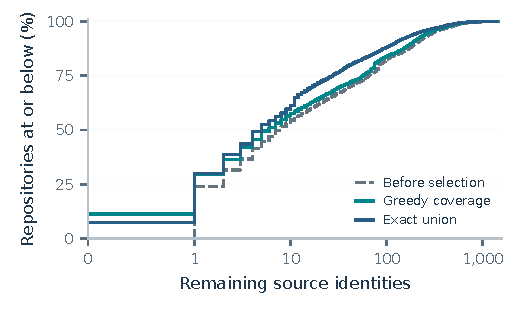
\includegraphics[width=\columnwidth]{source_multiplicity_compact.pdf}
\caption{Remaining sources at budget 100 over 7,158 source-reachable repositories. Zero remaining sources identify all-source exclusions. The horizontal scale is logarithmic above one.}
\label{fig:sources}
\end{figure}

\subsection{Selection Rules and Budget Grid}
We compare portfolio size, summed per-package reach, maximum per-package reach, exact portfolio-union reach, and greedy maximum marginal coverage. The sum baseline double-counts overlap within a portfolio. Greedy repeatedly adds the identity contributing the most newly covered endpoints. Coverage is monotone submodular, so this established method has the standard $1-1/e$ lower bound relative to optimal coverage~\cite{nemhauser1978}; that guarantee does not apply to $H$ or $P$. The additional exclusion-oriented heuristic has no global optimality guarantee.

Each rule produces nested selections at budgets $1,5,10,25,50,100$, with equal account costs and ascending usernames to break ties. The random baseline uses 200 seeded uniform orders without replacement; each order is reused across endpoint universes. Hypergeometric probabilities supply exact expectations from source multiplicities. Central 95\% simulation ranges describe variation between selections on this graph. They provide no population confidence interval for npm. We saved an exploratory analysis plan before execution, without external preregistration.

% Declare the wide budget plot early so it can float beside the results.
\begin{figure*}[t]
\centering
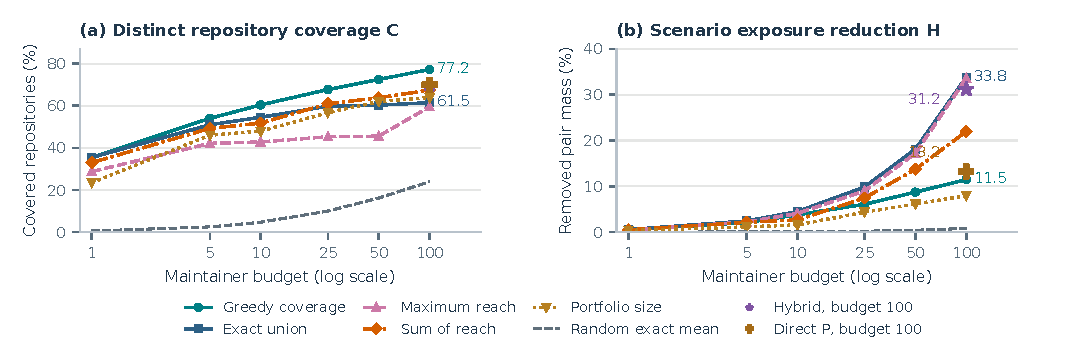
\includegraphics[width=\textwidth]{objective_tradeoff.pdf}
\caption{Workflow-repository coverage and conditional exposure reduction favor different selections. Lines connect the six evaluated budgets. The random curve is the exact expectation; stars and plus markers show the two additional budget-100 sensitivities.}
\label{fig:budget}
\end{figure*}

\subsection{Reproducibility and Checks}
The read-only Python implementation records hashes, seeds, environment, and definitions. Breadth-first searches independently verify 288 roots and all 25,228 stored package transitive counts; dual incidence, union bounds, nested curves, and $P\le C$ are checked. Tests cover cycles, version splicing, and 675 roots in 60 seeded small graphs. The grid contains 150 deterministic and 6,000 random budget rows across five endpoint/visibility definitions. No package payload is executed.

Three isolated full reruns reproduce aggregate results byte for byte. On Linux x86-64 with Python 3.14.8, mean wall time is 39.50 s (sample SD 0.98 s), with maximum peak RSS 1,038.4 MiB. These include extraction, baselines, sensitivities, and serialization; uncontrolled caches preclude online-cost inference.


\subsection{Additional Structural Sensitivities}
At budget 100, a hybrid greedily maximizes marginal gain of $J_\alpha(S)=\alpha C(S)/|U|+(1-\alpha)H(S)$ at $\alpha=0.50$. A separate heuristic lexicographically prioritizes immediately completed source sets, fractional remaining-source contributions, marginal coverage, and username order. Candidates come from endpoints with one to ten remaining sources, falling back to all unselected identities.

To distinguish the earlier residual threshold from strict exclusion, define $R_+=\{e:A_e\ne\varnothing\}$ and
\begin{equation}
 T_k(S)=|\{e\in R_+:|A_e\setminus S|<k\}|,\quad
 \Delta T_k=T_k(S)-T_k(\varnothing).
\end{equation}
$T_k$ is a residual-source count, not an enforced review quorum. The strict variant $P_k^{\rm strict}$ counts only endpoints with zero remaining sources or with $|A_e|\ge k$ and fewer than $k$ remaining sources. It has zero baseline; all 13 source-free endpoints are excluded. Uniform efficacy sensitivity $H_\eta=\eta H$ scales the stipulated exposure reduction without estimating a bypass rate.
